
%\section{Method}
%\begin{figure*}[t]
    \centering
    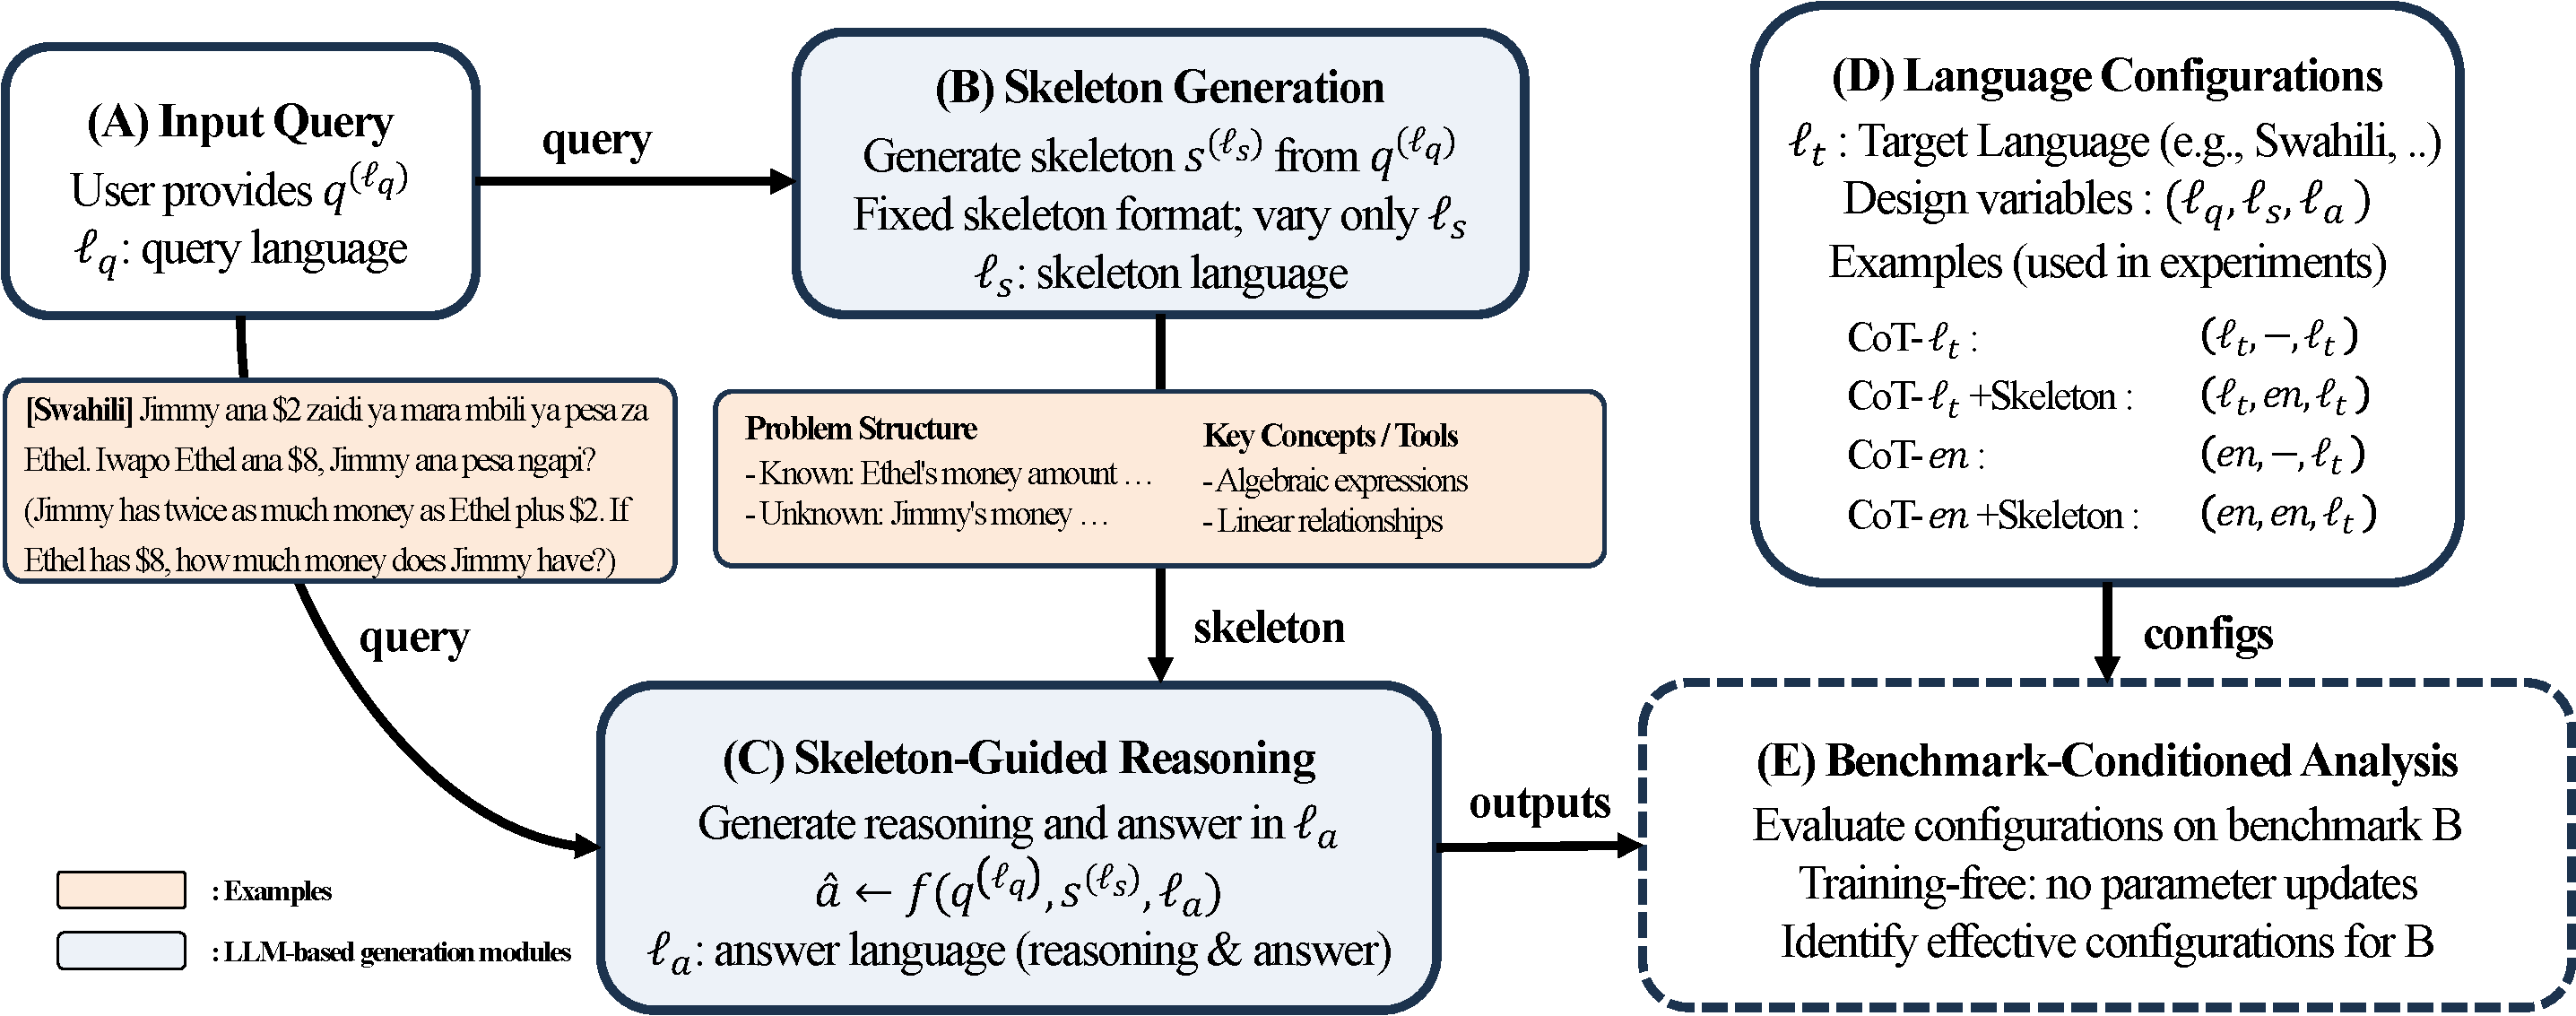
\includegraphics[width=\textwidth]{Figures/Images/LASOF3.pdf}
    \caption{\small Overview of the Skeleton-Guided Reasoning Framework. (A) The process begins with an input query $q^{(\ell_q)}$. (B) A structured skeleton $s^{(\ell_s)}$ is generated to abstract the problem logic. (C) The final reasoning and answer $\hat{a}$ are produced in the answer language $\ell_a$, conditioned on the query and skeleton. (D) We define the language configuration space as $(\ell_q, \ell_s, \ell_a)$ and compare four primary strategies: standard CoT and skeleton-guided approaches, applied in both the target language ($\ell_t$) and English ($en$). (E) Effective configurations are identified through training-free benchmark analysis.
}
\label{fig:figure1}
    \vspace{-0.15in}
\end{figure*}


%\paragraph{Overview}
%본 연구는 모델이 보유한 영어 기반의 추론 능력을 타겟 언어 생성 과정에 효과적으로 전이하는 것을 목표로 한다. 이를 위해 우리는 문제 해결을 위해 구조적 특성과 요구 개념을 영어로 추출한 \textsc{Skeleton}을 활용하는 \textsc{Skeleton-Guided Chain-of-Thought}를 제안한다. 
%해당 프레임워크는 \textsc{Skeleton}을 생성하는 첫 번째 단계(\S\ref{sec:stage1-skeleton-generation})와, \textsc{Skeleton}을 활용하여 CoT를 진행하는 두 번째 단계(\S\ref{sec:stage2-skeleton-cot})로 구성된다.

%\subsection{Stage 1: Skeleton Generation}
%\label{sec:stage1-skeleton-generation}
%ST-CoT의 첫 번째 단계는 특정 언어로 주어진 질문 $L_t$로부터 문제 해결에 필요한 핵심 구조적 요소만을 추출한 Skeleton을 생성하는 과정이다. 이 단계에서는 언어적 표현이나 서술 방식에 종속되지 않으면서, 문제의 논리적 구조와 개념적 관계만을 안정적으로 추출하여 $L_t$에서의 추론 과정에 견고한 논리적 기반을 제공하도록 한다.

%Skeleton 생성을 위한 식은 다음과 같다:

%\begin{equation}
%    S = M(q_{L_t}; P_{\text{sys}}, \mathcal{E}),
%    \label{eq:skeleton_generation_revised}
%\end{equation}

%여기서 $M$은 Instruction-tuned LLM을 의미하며, $P_{\text{sys}}$는 Skeleton 생성 원칙을 명시한 시스템 프롬프트이다. $\mathcal{E}$는 In-context learning을 위한 Few-shot 예제 집합이다.
%이때 핵심적인 전략은 Cross-lingual Skeleton Alignment이다. 입력 질문 $q_{L_t}$는 타겟 언어로 주어지지만, 출력인 $S$는 모델의 추론 능력이 가장 강력한 영어로 생성되도록 강제한다. 이를 통해 모델의 가장 안정적인 추론 공간인 영어에서 고수준의 논리 구조를 설계할 수 있다.
%\subsection{Stage 2: Skeleton-Guided CoT}
%\label{sec:stage2-skeleton-cot}



%\section{Language-Aware Skeleton Optimization Framework}

%\subsection{Problem Setup and Language Dimensions}

%본 연구는 다국어 환경에서 스켈레톤 기반 추론이 어떠한 언어 설정 하에서 효과적으로 작동하는지를 분석하는 것을 목표로 한다. 이를 위해 우리는 스켈레톤의 형식이나 구조를 변경하지 않고, 언어 선택에 따른 추론 성능 변화를 분리하여 관찰할 수 있는 문제 설정을 채택한다.

%하나의 문제 인스턴스는 질의 $q$와 이에 대한 정답 $a$로 구성되며, 질의는 특정 언어 $\ell_q \in \mathcal{L}$로 주어진다. 여기서 $\mathcal{L}$은 실험에 포함된 언어들의 집합을 의미한다. 모델은 질의 $q$를 입력으로 받아 중간 추론 과정 $r$과 최종 답변 $\hat{a}$를 생성한다. 스켈레톤 기반 추론에서는, 중간 추론 $r$이 직접 생성되기 이전에, 문제 해결을 위한 간결한 구조적 가이드인 스켈레톤 $s$가 먼저 생성된다.

%다국어 스켈레톤 기반 추론 파이프라인은 다음 세 가지 언어 선택을 포함한다.
%\begin{itemize}
%    \item \textbf{질의 언어} $\ell_q$: 사용자가 질의를 작성하는 언어
%    \item \textbf{스켈레톤 언어} $\ell_s$: 문제 해결의 구조를 표현하는 스켈레톤이 생성되는 언어
%    \item \textbf{추론 및 답변 언어} $\ell_r$: 상세 추론 과정과 최종 답변이 생성되는 언어
%\end{itemize}

%이 세 언어는 동일할 수도 있고 서로 다를 수도 있으며, 각각의 선택에 따라 모델이 활성화하는 언어적 prior와 추론 경로가 달라질 수 있다. 따라서 하나의 스켈레톤 기반 추론 과정은 언어 조합 $(\ell_q, \ell_s, \ell_r)$로 정의될 수 있다.

%본 연구에서는 스켈레톤의 구조와 생성 방식은 고정한 채, 언어 조합에 따른 영향을 분석하는 데 초점을 둔다. 이를 통해 스켈레톤 기반 추론 성능을 다음과 같이 표현한다.
%\[
%\hat{a} = f(q^{(\ell_q)}, s^{(\ell_s)}, \ell_r),
%\]
%여기서 $f(\cdot)$는 사전 학습된 언어 모델의 추론 함수를 나타내며, $s^{(\ell_s)}$는 언어 $\ell_s$로 표현된 스켈레톤이다.

%특히 본 연구는 두 가지 실용적인 설정에 주목한다. 첫째, 질의 언어와 추론 언어를 동일하게 유지한 채 $(\ell_q = \ell_r)$ 스켈레톤 언어 $\ell_s$만을 변화시키는 설정이다. 이는 번역 없이 스켈레톤을 활용하는 경우를 모델링한다. 둘째, 질의 언어를 영어로 변환한 후 $(\ell_q = \text{en})$ 추론을 수행하는 설정으로, 영어 피벗 추론(TransEN)을 반영한다. 이 두 설정을 통해 우리는 스켈레톤이 번역을 대체하거나 보완할 수 있는 조건을 체계적으로 비교할 수 있다.

%중요하게도, 본 절에서 정의한 언어 조합에 대한 분석은 새로운 학습이나 파라미터 업데이트를 포함하지 않는다. 이후 절에서는 이러한 문제 설정을 바탕으로, 구체적인 언어 구성 방식과 스켈레톤 활용 방법을 설명한다.


\begin{figure*}[t]
    \centering
    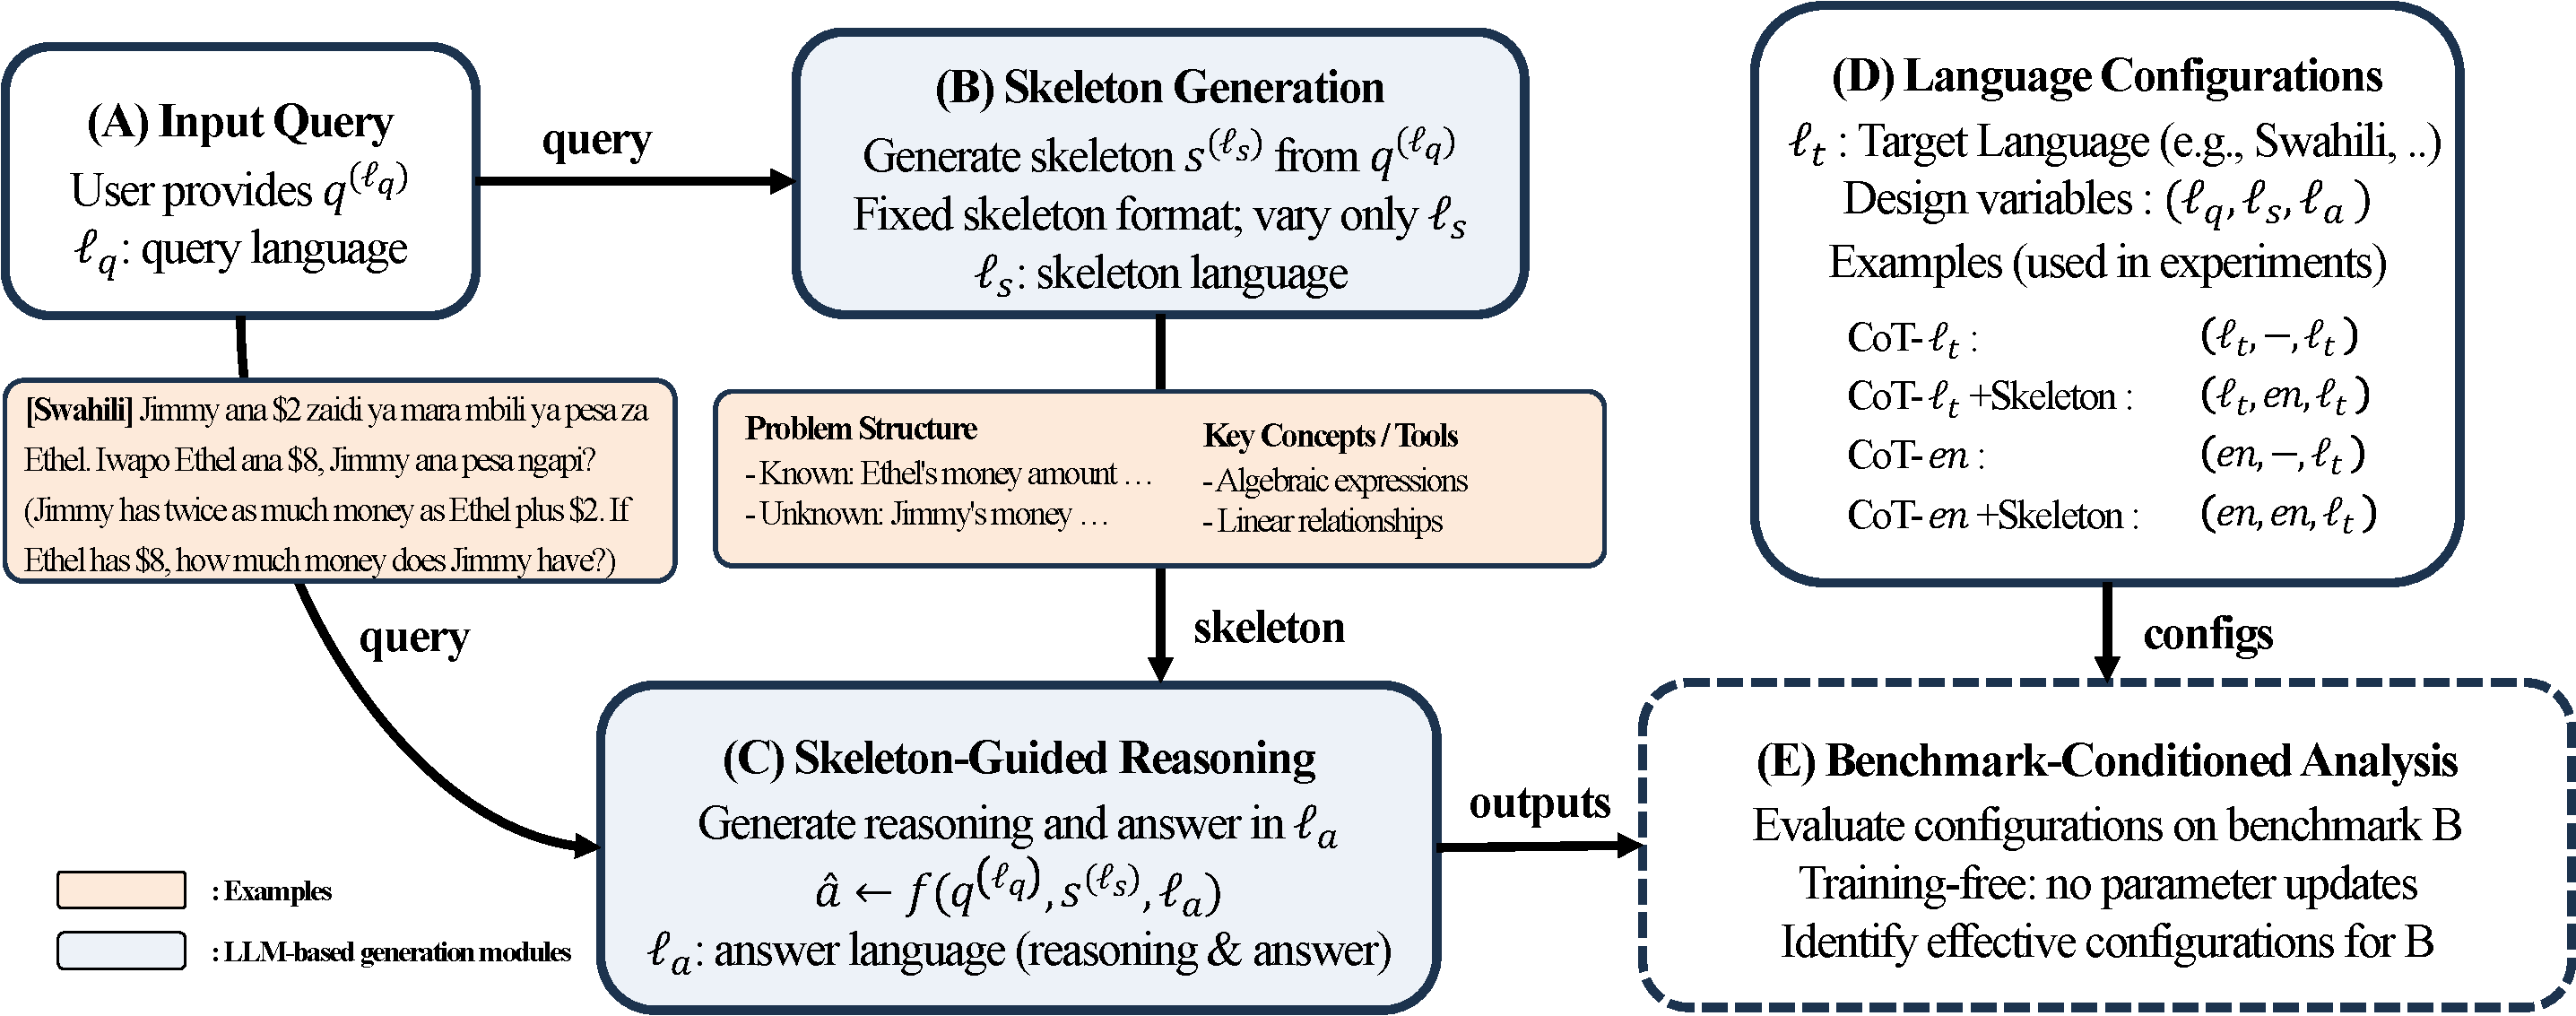
\includegraphics[width=\textwidth]{Figures/Images/LASOF3.pdf}
    \caption{\small Overview of the Skeleton-Guided Reasoning Framework. (A) The process begins with an input query $q^{(\ell_q)}$. (B) A structured skeleton $s^{(\ell_s)}$ is generated to abstract the problem logic. (C) The final reasoning and answer $\hat{a}$ are produced in the answer language $\ell_a$, conditioned on the query and skeleton. (D) We define the language configuration space as $(\ell_q, \ell_s, \ell_a)$ and compare four primary strategies: standard CoT and skeleton-guided approaches, applied in both the target language ($\ell_t$) and English ($en$). (E) Effective configurations are identified through training-free benchmark analysis.
}
\label{fig:figure1}
    \vspace{-0.15in}
\end{figure*}

\section{Language-Aware Skeleton Exploration Framework}
% \section{Language-Aware Skeleton Optimization Framework}

본 연구는 다국어 환경에서 스켈레톤 기반 추론의 효과가 언어 선택과 평가 환경에 따라 어떻게 달라지는지를 분석하는 것을 목표로 한다. 이를 위해 우리는 스켈레톤의 구조나 형식은 고정한 채, 언어 설정만을 변화시키는 방식으로 스켈레톤 활용을 체계적으로 분석하는 \emph{Language-Aware Skeleton Exploration Framework (\LASEF)}를 제안한다. 여기서 `탐색'란 새로운 학습이나 알고리즘적 탐색을 의미하는 것이 아니라, 주어진 평가 환경에서 효과적인 언어 구성을 식별하는 경험적 분석 과정을 의미한다.

% 여기서 `최적화'란 새로운 학습이나 알고리즘적 탐색을 의미하는 것이 아니라, 주어진 평가 환경에서 효과적인 언어 구성을 식별하는 경험적 분석 과정을 의미한다.

\subsection{Problem Setup and Language Dimensions}


일반적으로 언어 모델의 활용은 질의 $q$와 이에 대한 답변 $a$로 구성되며, 질의는 특정 언어 $\ell_q$로 주어진다. 스켈레톤 기반 추론에서는 모델이 먼저 질의를 바탕으로 문제 해결에 필요한 핵심 구조를 요약한 스켈레톤 $s$를 생성하고, 이를 활용하여 상세한 추론 과정과 최종 답변을 생성한다. 이 과정에는 세 가지 언어 선택이 관여한다: 사용자의 target 언어 $\ell_t$ 가 있을때, (1) 질의가 표현되는 언어 $\ell_q$, (2) 스켈레톤이 표현되는 언어 $\ell_s$, (3) 상세 추론 및 최종 답변이 생성되는 언어 $\ell_a$.

이 세 언어는 동일할 수도 있고 서로 다를 수도 있으며, 그 조합에 따라 모델이 활성화하는 언어적 prior와 추론 경로가 달라질 수 있다. 따라서 하나의 스켈레톤 기반 추론 과정은 언어 조합 $(\ell_q, \ell_s, \ell_a)$로 특징지을 수 있다. \LASEF는 스켈레톤의 생성 방식과 구조를 고정한 채, 이러한 언어 조합이 추론 성능에 미치는 영향을 분리하여 분석하는 데 초점을 둔다. 이를 통해 스켈레톤 기반 추론 과정을 다음과 같이 표현할 수 있다:
\[
\hat{a} = f\big(q^{(\ell_q)}, s^{(\ell_s)}, \ell_a\big),
\]
여기서 $f(\cdot)$는 사전 학습된 언어 모델의 추론 함수를 나타내며, $s^{(\ell_s)}$는 언어 $\ell_s$로 표현된 스켈레톤이다.

중요하게도, 스켈레톤 활용에서 효과적인 언어 조합은 보편적으로 고정되어 있지 않으며, 평가 기준이 되는 벤치마크나 도메인에 따라 달라질 수 있다. 특정 벤치마크 $B$가 질의–정답 쌍의 집합으로 주어질 때 $(\{q,a\} \in B)$, LASEF는 다양한 언어 조합 $(\ell_q, \ell_s, \ell_a)$ 하에서의 성능 변화를 비교함으로써, 해당 평가 환경에서 상대적으로 효과적인 스켈레톤 언어 구성을 식별하는 분석 프레임워크를 제공한다.

본 문제 설정은 추가 학습이나 파라미터 업데이트를 포함하지 않는 \emph{training-free} 환경을 전제로 한다. 다음 절에서는 이러한 설정을 바탕으로, 본 연구에서 고려하는 구체적인 언어 구성과 스켈레톤 활용 방식을 설명한다.

\subsection{Skeleton Construction and Usage}

본 연구에서 사용하는 스켈레톤은 문제 해결에 필요한 핵심 정답이나 계산 절차를 제시하는 것이 아니라, 문제 풀이를 위한 \emph{사고의 구조(thinking structure)}를 간결하게 드러내는 중간 표현이다. 즉, 스켈레톤은 추론 과정이 따라야 할 최소한의 구조적 가이드를 제공하되, 실제 해결 과정에 대한 구체적인 지침은 포함하지 않는다. 이러한 관점은 스켈레톤을 문제 해결의 요약이나 힌트가 아닌, 추론을 조직하는 구조적 표현으로 해석하는 기존 연구 흐름과 개념적으로 정렬된다.

이에 따라 본 연구의 스켈레톤은 매우 짧고 추상적인 형태를 유지하며, 문제의 구체적인 계산 단계나 정답을 포함하지 않는다\footnote{Using longer skeletons risks leaking solution strategies into the prompt, which would confound our goal of isolating the effect of language choice from that of explicit reasoning supervision.}. 이를 명확히 하기 위해, 스켈레톤 생성 시 다음 원칙을 일관되게 적용한다: \emph{``Provide only the essential structural characteristics of the problem. Describe what the problem structure is, never how to solve it.''}

Figure~\ref{fig:figure1}은 본 연구에서 사용된 스와힐리어 질의($\ell_q=sw$)에 대해 영어로 생성된 스켈레톤($\ell_s=en$)의 대표적인 예시를 보여준다. 제안한 기준에 따라 생성된 스켈레톤은 언어에 관계없이 평균적으로 약 n 토큰 내외의 짧은 길이를 가지며, 정답이나 핵심 풀이 과정을 직접적으로 포함하지 않는다. 이러한 특성은 단일 예제에 국한되지 않으며, 스켈레톤 길이와 내용 분포에 대한 정량적 분석은 Section~\ref{}에서 보고한다. 또한 전체 스켈레톤 생성 규칙과 추가 예제는 Appendix~\ref{}에 제시한다.

%중요하게도, 본 연구의 모든 실험 설정에서 스켈레톤의 형식과 생성 원칙은 동일하게 유지되며, 언어 선택만을 변화시킨다. 이를 통해 스켈레톤의 구조적 설계와 언어 조합의 효과를 분리하여 분석할 수 있으며, 이후 실험에서는 언어 설정에 따른 추론 성능 변화가 스켈레톤의 내용 자체가 아닌 언어적 요인에 기인함을 검증한다.

%\subsection{Language Configurations for Skeleton-Guided Reasoning}

%이번 장에서는 3.1절에서 LASOF에 적용할 언어 조합 $(\ell_q,\ell_s,\ell_t)$을 실제 어떻게 구체화하였는지 서술한다. %모든 설정에서 스켈레톤의 형식과 생성 방식은 동일하게 유지되며, 언어 조합만을 변화시킨다. %이를 통해 벤치마크 $B$에 조건화된 언어 구성의 효과를 다른 요인과 분리하여 관찰할 수 있다.

%\paragraph{Target-Language CoT (CoT).}
%기본 설정으로, 질의와 추론 및 답변이 동일한 target 언어로 이루어진다 $(\ell_q=\ell_t)$. 이 경우 모델은 일반적인 Chain-of-Thought 프롬프트를 사용하여 번역 없이 직접 추론을 수행해 baseline환경이 된다.

%\paragraph{Target-Language CoT with Skeleton (+Skeleton).}
%질의와 추론 언어는 target 언어로 유지하되 $(\ell_q=\ell_t)$, 스켈레톤을 제공한다 $(\ell_s=\text{en})$. 이 설정은 번역 없이도 영어 중심 추론 prior를 구조적 가이드 형태로 활용할 수 있는지를 평가한다.

%\paragraph{English-Pivot Reasoning (TransEN).}
%질의를 영어로 변환한 뒤 $(\ell_q=\text{en})$, 영어로 추론과 답변을 생성하는 설정이다. 이는 영어 중심으로 사전학습된 LLM에서 널리 사용되는 강력한 비교 기준에 해당한다.

%\paragraph{English-Pivot Reasoning with Skeleton (TransEN + Skeleton).}
%질의와 스켈레톤 모두 영어로 제공하는 설정이다 $(\ell_q=\ell_s=\text{en})$. 이 구성은 영어 피벗 환경에서 스켈레톤이 추가적인 구조적 이점을 제공하는지를 평가하기 위한 상한선 역할을 한다.

%이 네 가지 언어 구성은 LASOF가 정의하는 언어 조합 공간의 대표적인 부분집합으로, 이후 실험에서는 각 벤치마크 $B$에 대해 이러한 구성들이 보이는 상대적 경향을 비교·분석한다.

